\documentclass[a4paper, twocolumn]{article}
\usepackage[utf8]{inputenc}
\usepackage{graphicx}
\usepackage{url}

\title{Obstacle avoidance and target acquisition with an event-based camera on a neuromorphic chip}
\author{Alexander Dietmüller \& Hermann Blum \\INILabs\\ETH Zürich}
\date{October 2016}

\begin{document}

\maketitle

\section*{Introduction}
Navigation through an unknown environment is a standard problem in robotics and includes target acquisition and obstacle avoidance. The wide variety of solutions depends on the choice of sensors and on the computing architecture. 

If a map of the environment is known, target acquisition amounts to the problem of planning an optimal route from the starting to the target position on the map. If the map of the environment is not known, the problem of simultaneous localisation and mapping (SLAM) is considered.  In reactive approaches to navigation, the robot updates its trajectory depending on the current readings of its sensors, without planning the whole route in advance. In these approaches, the robot stays flexible and quickly adapts to changes in the environment, e.g. the moving obstacles.  Potential field and dynamical systems approaches are two reactive approaches to robotic navigation. The dynamical systems approach has been proven to be an effective low level, reactive solution for obstacle avoidance and target acquisition \cite{bicho1998}.A particular, neurally-inspired flavour of the dynamical systems approach -- the Dynamic Neural Fields (DNF) framework -- has been useful in the design of autonomous cognitive robots \cite{erlhagen2006}. In particular, for robot navigation, DNFs were used to hold representation of the direction towards the target in working memory \cite{bicho2000}.
 
In reactive approaches, information about the obstacles and the target has to be updated based on the sensor readings faster than the relaxation time constant of the dynamics. Thus, using  the biologically inspired Dynamic Vision Sensor (DVS) \cite{lichtsteiner2008} offers an advantage of real-time (very fast) processing of sensory information, enabling reactive navigation at high speed. The DVS can be used as direct input to the DNFs \cite{sandamirskayaconradt2013} In this project, we will enable fast processing of the DVS events for detection of obstacles and the target by implementing a DNF-like architecture in neuromorphic hardware, enabling real-time processing of the incoming spikes and minimising delays. The work of Frising \cite{frising} has validated that this approach is suitable for the desired task.

The neuromorphic VLSI implementations of spiking neurons offer low power consumption and real-time processing \cite{indiveri2011}. The neuromorphic Re-configurable OnLine Learning System (ROLLS) \cite{qiao2015} developed at INI will be the core platform, which, combined with the DVS, forms a fast and low-power consuming architecture for autonomous robots. We may additionally use digital designs, which offer greater flexibility and more neurons.

\newpage

\section*{Objective}
This work will combine basic functionalities like obstacle avoidance and target acquisition with a decision-making using DNFs in a small spiking neural network. The robot will therefore be able to move around an obstacle, keep the angular position of the target in memory, and  return to the target acquisition task after the obstacle avoidance maneuver. We will test the target acquisition architecture with a localised target and a line, which the robot will follow. 

The system will be optimized towards fast and fluent action by using the DVS sensor and the ROLLS chip. This work will explicitly not focus on more complex processing of the DVS input signal (e.g., object recognition) as well as hardware development.
In the following, we describe the different project phases and objectives in detail.

\section*{First Phase: Exploring the platforms and framework}
We will first use the framework by Michel Frising to get familiar with the hardware (ROLLS and CXQUAD chip, DVS camera) and software frameworks and interfaces (cAER, aerctl, NCSRobotLib, etc.) and combine the basic solutions of target acquisition and obstacle avoidance.
The NCSRobotLib offers  a basic software framework of ``devices’’ (event emitters) and ``listeners’’, which implement different controllers and communication interfaces between devices. We will consider using Qt and ROS frameworks to enable communication between different devices, preferring the most ``light-weight’’ solution which may be embedded on a mobile computing platform. This work will be performed using the pushbot platform. The pushbots are small robots equipped with a DVS camera. [Figure \ref{fig:pushbot}] \cite{pushbot}.

\begin{figure}
    \centering
    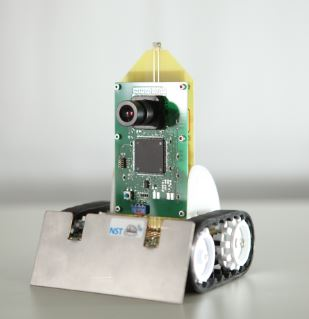
\includegraphics[width=1.0\linewidth]{pushbot1croppedcropped.jpg}
    \caption{The pushbot platform developed by Prof. Jörg Conradt and team at the Neuroscientific System Theory group of the Technical University of Munich}
    \label{fig:pushbot}
\end{figure}

\section*{Second Phase: Attractors, Obstacle Avoidance \& DNF}
First of all, we will improve the target representation of Frising’s project, in which a discrete discrimination between ``left’’, ``right’’ and ``center’’ was used, and transform this into a continuous representation of the target position. Subsequently, we will add a ``high level’’ decision network (with DNF) to decouple target following and obstacle avoidance behaviors and to enable a decision-making process about deviation from the trajectory towards the target. This will include keeping the target position memorized while performing obstacle avoidance.
The obstacle avoidance, implemented by Frising, amounts to clutter detection in the lower part of the DVS image, and will be improved in this work.

\section*{Third phase: Robotic experiments and documentation}
Finally, we will perform experiments in a simplified, but close to natural, office environment, recoding the robot’s trajectory and quantitatively validating obstacle avoidance and target acquisition behaviors. 

The results of the project will be documented in a final report.

\newpage

\section*{Time schedule}
\newcounter{remember}
\begin{itemize}
    \item[] Planning and Preparation (2 Weeks)
    \begin{enumerate}
        \item Reading
        \item Project proposal and discussion
        \setcounter{remember}{\value{enumi}}
    \end{enumerate}
    
    \item[] First phase (3 Weeks)
    \begin{enumerate}
        \setcounter{enumi}{\value{remember}}
        \item Familiarisation with neuromorphic hardware, DVS-based vision and frameworks
        \item Combining existing obstacle avoidance and target acquisition
        \item Finishing first phase, experiment recording and documentation
        \setcounter{remember}{\value{enumi}}
    \end{enumerate}
    
    \item[] Second phase (6 Weeks)
    \begin{enumerate}
        \setcounter{enumi}{\value{remember}}
        \item Refining target acquisition (continuous position)
        \item Refining obstacle avoidance (if necessary)
        \item Design of DNF networks
        \item Decision making between target acquisition and obstacle avoidance
        \item Keeping target position in memory, position dependent on motor movement
        \item time buffer, potentially also used for speed and power optimization
        \setcounter{remember}{\value{enumi}}
    \end{enumerate}
    
    \item[] Third Phase (3 Weeks)
    \begin{enumerate}
        \setcounter{enumi}{\value{remember}}
        \item Report writing
        \item Christmas holidays / time buffer
        \item Recording of experiments
    \end{enumerate}
\end{itemize}	


\bibliographystyle{apalike}
\bibliography{literature}

\end{document}
